\chapter{Estructura primaria o secuencia} \label{secuencia}

En estas secciones veremos dos ejemplos de algoritmos que utilizan secuencias de DNA y prote\'\i{}nas con el objeto de estudiar procesos que dependen de propiedades estructurales.

%\section{Estabilidad y deformaci\'{o}n de un d\'{u}plex de ADN: predicci\'{o}n de promotores} \label{dna1}
 
 
El modelo \italics{Nearest Neighbor} (NN) aproxima la estabilidad termodin\'{a}mica de un \'{a}cido nucleico en disoluci\'{o}n
a partir de su secuencia, que se analiza como una secuencia de dinucle\'{o}tidos solapantes 
de interacciones aditivas, cuyas energ\'{i}as se han determinado experimentalmente \citep{Breslauer1986,SantaLucia1998}.

\begin{figure}
\begin{center} 
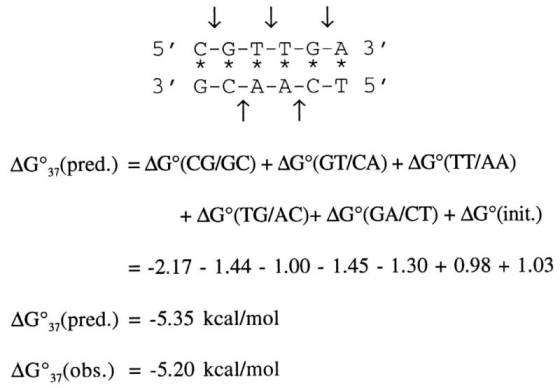
\includegraphics{NN}
\caption
{
C\'{a}lculo de estabilidad (energ\'{i}a libre de Gibbs, $\Delta G$) a temperatura fisiol\'{o}gica en base al modelo NN, 
incluyendo un t\'{e}rmino de iniciaci\'{o}n de d\'{u}plex, tomado de \citep{SantaLucia1998}.
Copyright (1998) National Academy of Sciences.
}
\label{fig:NN}
\end{center}
\end{figure}

Inspir\'{a}ndose en estructuras moleculares conocidas, 
este tipo de modelos se han empleado para describir la lectura indirecta del DNA, por su forma, 
por parte de nucleosomas \citep{Heijden2012} o factores de transcripci\'{o}n \citep{Gromiha2004,Espinosa2008}.

\begin{figure}
\begin{center} 
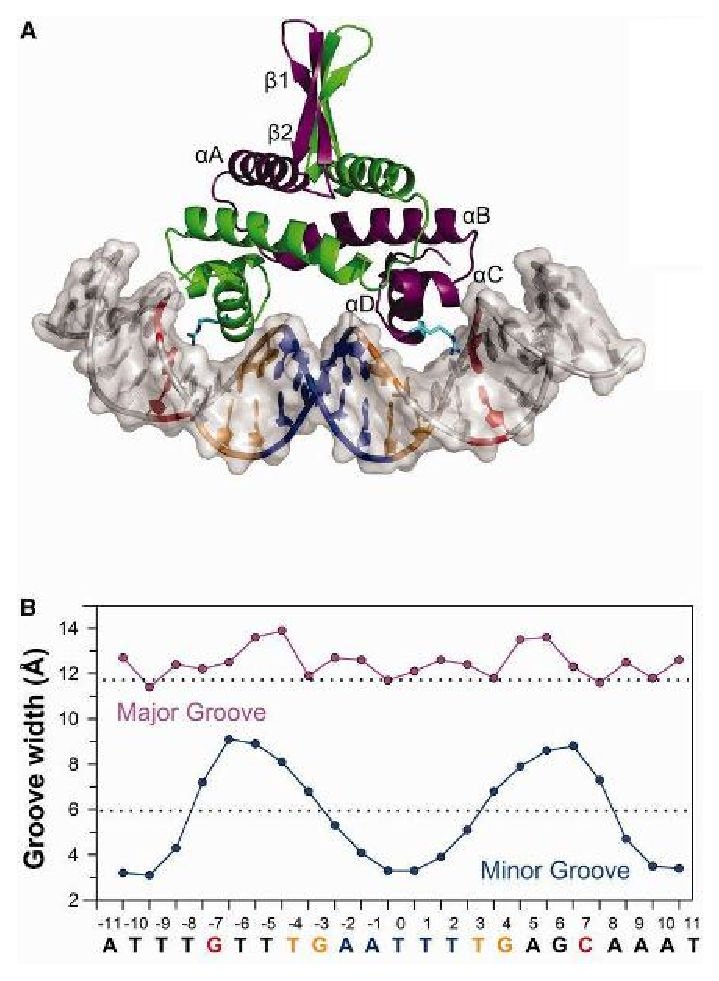
\includegraphics{MGW}
\caption
{
(A) Estructura de un homod\'{i}mero de Fis unido a un sitio de alta afinidad 
(PDB: \htmladdnormallink{3IV5}{http://www.rcsb.org/structure/3IV5}), 
insertando dos h\'{e}lices en dos surcos mayores consecutivos. 
(B) Ancho del surco mayor (magenta) y menor (MGW, azul) a lo largo de la secuencia de DNA medido entre los fosfatos m\'{a}s cercanos.
Las lineas punteadas representan los valores can\'{o}nicos para B-DNA. 
Figura adaptada de \citet{Hancock2013} y reproducida con permiso de los autores.
}
\label{fig:MGW}
\end{center}
\end{figure}

\begin{figure}
\begin{center} 
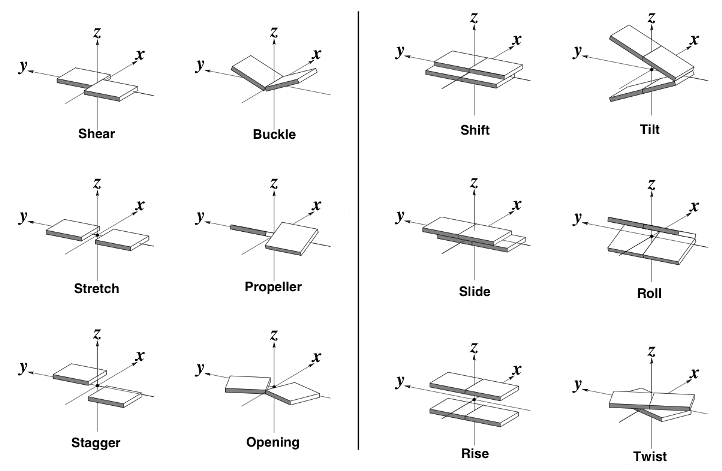
\includegraphics{BPgeom}
\caption
{
Propiedades de pares de bases (izquierda) y dinucle\'{o}tidos (derecha) que se pueden estimar a partir de la estructura. 
Figura tomada de \htmladdnormallink{x3dna.org}{http://x3dna.org/articles/seeing-is-understanding-as-well-as-believing}.
}
\label{fig:BPgeometry}
\end{center}
\end{figure}

%\begin{figure}
%\begin{center} 
%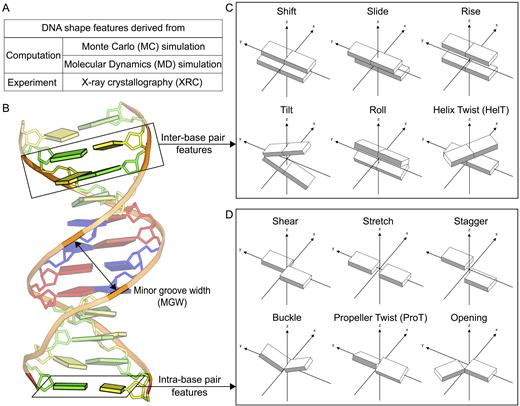
\includegraphics{DNAshape13}
%\caption{Propiedades de pares de bases y dinucle\'{o}tidos que se pueden estimar a partir de la estructura \citep{Li2017}.}
%\label{fig:DNAshape13}
%\end{center}
%\end{figure}



Otros modelos ampl\'{i}an el n\'{u}mero de vecinos considerados hasta llegar, por ejemplo, a pent\'{a}meros:

\begin{figure}
\begin{center} 
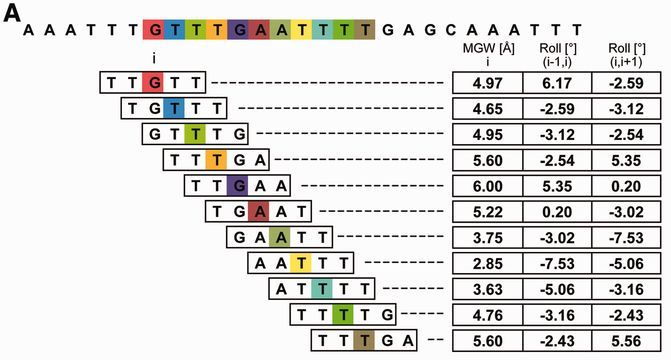
\includegraphics{DNApentamers}
\caption
{
Aproximaci\'{o}n de propiedades estructurales (MGW=minor groove width) de un d\'{u}plex de ADN por solapamiento de pent\'{a}meros, 
base del algoritmo \htmladdnormallink{DNAshape}{http://rohsdb.cmb.usc.edu}. 
Reproducido con permiso de \citet{Zhou2013}.
Este tipo de aproximaciones se est\'{a}n usando para enriquecer motivos de DNA reconocidos por factores de transcripci\'{o}n \citep{Yang2015}.
}
\label{fig:NN5}
\end{center}
\end{figure}

En esta secci\'{o}n aplicaremos el modelo NN a la predicci\'{o}n de promotores:

\begin{itemize}
\item \textbf{PROBLEMA:} disponemos de coordenadas gen\'{o}micas de una colecci\'{o}n de marcos de lectura 
(\htmladdnormallink{\italics{Open Reading Frames, ORFs}}{http://es.wikipedia.org/wiki/Marco_abierto_de_lectura}), 
pero desconocemos la posici\'{o}n de sus secuencias promotoras
\item \textbf{SOLUCI\'{O}N PROPUESTA:} buscar los promotores en la secuencia del DNA por su menor estabilidad termodin\'{a}mica
\end{itemize}

Este problema ha tenido mayor importancia en procariotas por la gran velocidad con que se han ido obteniendo sus secuencias gen\'{o}micas, 
y el algoritmo de \cite{Kanhere2005} es un ejemplo de como emplear una estrategia estructural para atacar este problema. 
El algoritmo consiste en estimar la estabilidad helicoidal del ADN cromos\'{o}mico, que se supone es menor en
las regiones promotoras, donde la maquinaria transcripcional se asienta para comenzar la s\'{i}ntesis de ARN. 
En concreto este m\'{e}todo estima la estabilidad de una (ventana de) secuencia de ADN a ambos lados de una coordenada y define como posibles
posiciones promotores aquellas donde la diferencia de estabilidad en torno a una coordenada es significativa. 

\begin{figure}
\begin{center} 
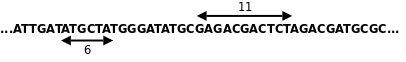
\includegraphics{window}
\caption
{
Ejemplos de ventanas de 6 y 11 nucle\'{o}tidos, que sirven para promediar propiedades a lo largo de la secuencia.
}
\label{fig:window}
\end{center}
\end{figure}

Este algoritmo incluye varios par\'{a}metros libres y en el art\'{i}culo original se muestra como entrenarlo para obtener valores adecuados para todos ellos.

\begin{figure}
\begin{center} 
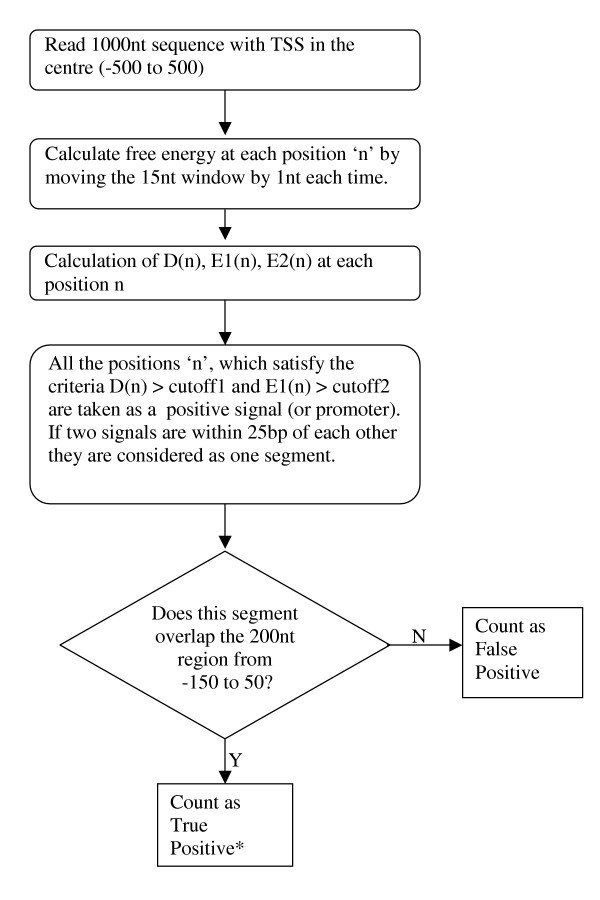
\includegraphics{flowKanhere}
\caption
{
Algoritmo de \cite{Kanhere2005}, que se basa en calcular la diferencia de $\Delta G$ entre dos ventanas en torno a una posici\'{o}n $n$.
Figura reproducida con permiso de los autores.
}
\label{fig:Kanhere}
\end{center}
\end{figure}

Se han propuesto otras aproximaciones estructurales, como la de \cite{Gogni2007}, %(\htmladdnormallink{PDF}{./papers/euk_promoter_prediction2007.pdf})
que identifica regiones promotoras en base a la capacidad de deformaci\'{o}n de los 
\htmladdnormallink{pares de bases}{http://nar.oxfordjournals.org/content/31/17/5108/F1.large.jpg},
estimada por medio de extensas simulaciones moleculares precalculadas. 
%Sin duda \'{e}sta es un \'{a}rea de investigaci\'{o}n en crecimiento y constantemente se siguen publicando 
%\htmladdnormallink{nuevos trabajos}{http://www.ncbi.nlm.nih.gov/pubmed?term=structural[All Fields] AND prediction[All Fields] AND promoters[All Fields]}. 

El repertorio de m\'{e}todos para predicci\'{o}n de promotores en base a inferencias estructurales es limitado, pero incluye al menos: 
\htmladdnormallink{proStar}{http://mmb.pcb.ub.es/proStar/}, \htmladdnormallink{ProSOM}{http://bioinformatics.psb.ugent.be/software/details/ProSOM}
%\htmladdnormallink{profisi}{http://mlg.ucd.ie/profisi} 
o el algoritmo de \citet{Song2012}. Otras opciones recientes se basan en combinar diferentes fuentes por medio de algoritmos de aprendizaje \citep{Eser2016}.

El ejercicio de esta secci\'{o}n consiste en completar el siguiente programa, usando los par\'{a}metros unificados de \cite{SantaLucia1998},
para calcular la diferencia de estabilidad $D(n)$ entre dos fragmentos de 50bp y 100bp $E1(n)$ y $E2(n)$ 
que flanquean una regi\'{o}n central (de 50bp) que podr\'{i}a albergar el promotor.
A su vez, estos framentos se calculan sobre valores de estabilidad calculados sobre ventanas de secuencia 
de longitud 15pb en el art\'{i}culo de \cite{Kanhere2005}:

\begin{equation}
E1(n) = \frac{\sum_{n}^{n+49}\Delta G}{50} 
\end{equation}

\begin{equation}
E2(n) = \frac{\sum_{n+99}^{n+199}\Delta G}{100} 
\end{equation}

\begin{equation}
D(n) = E1(n) - E2(n)
\end{equation}

Como conjunto de datos para la predicci\'{o}n de promotores usaremos las secuencias del fichero \htmladdnormallink{K12\_400\_50\_sites}{./files/K12_400_50_sites}, 
que contiene coordenadas de ORFs de \italics{Escherichia coli} con coordenadas -400,+50, con el 0 centrado cerca del cod\'{o}n de inicio.
Qu\'{e} observas al cambiar el tama\~no de la ventana?
\verbatiminput{code/prog1.1.pl}
  %estabilidad y deformacion de duplex de ADN y prediccion de promotores
%\section{Dise\~no de primers para PCR} \label{dna2}

La reacci\'{o}n en cadena de la polimerasa 
(\htmladdnormallink{PCR}{http://es.wikipedia.org/wiki/Reacci\%C3\%B3n_en_cadena_de_la_polimerasa})
es una metodolog\'{i}a est\'{a}ndar en cualquier laboratorio de biolog\'{i}a molecular y consta fundamentalmente
de 3 fases que se repiten un n\'{u}mero de ciclos dentro de un tubo de ensayo que se encuentra en un ba\~{n}o:

\begin{figure}
\begin{center} 
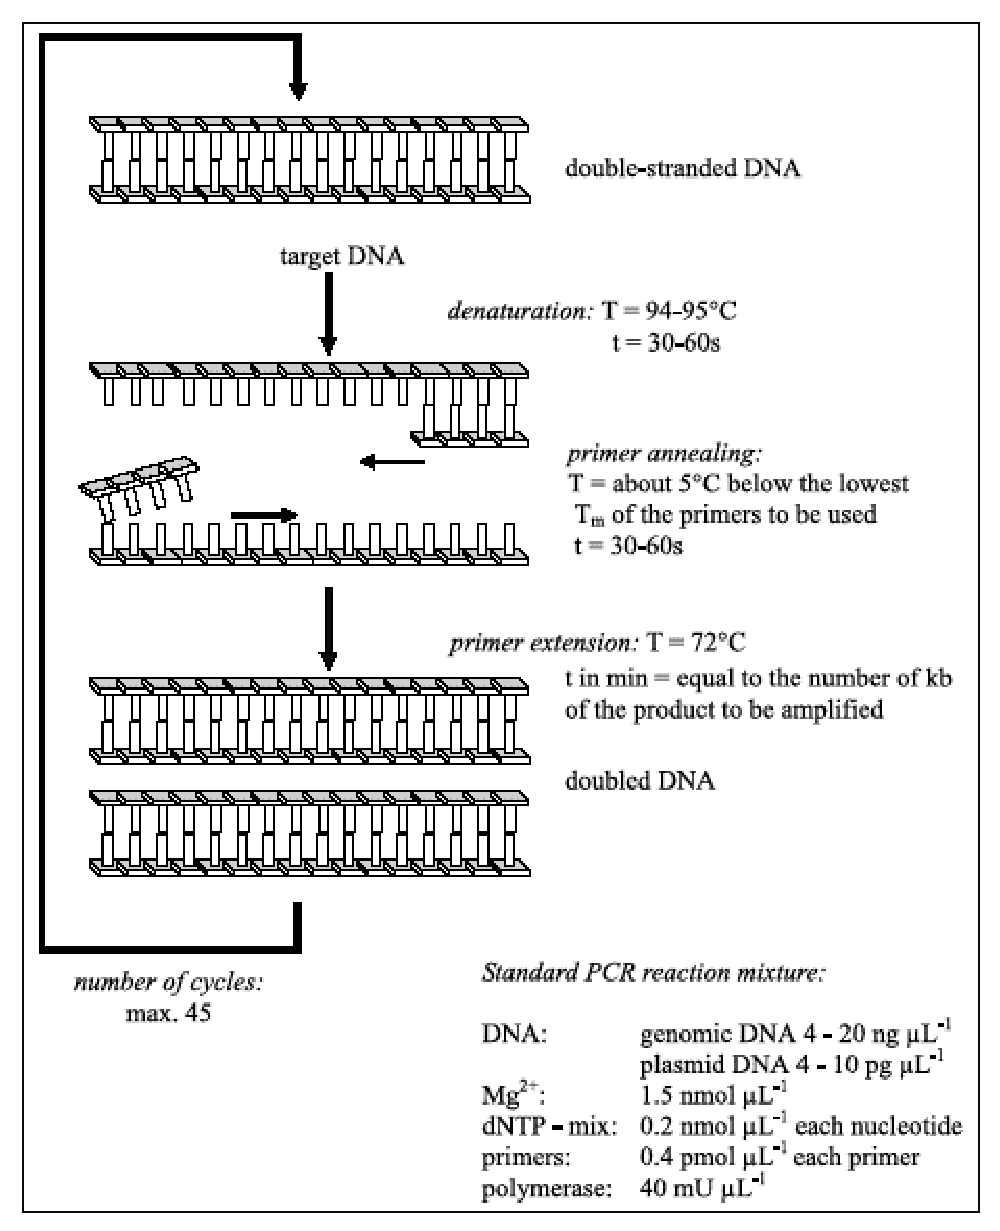
\includegraphics{PCR}
\caption
{
Diagrama de flujo de una reacci\'{o}n de PCR, 
que consiste en ciclos donde se repiten 3 fases: desnaturalizaci\'{o}n, apareamiento y elongaci\'{o}n.
En la primera el ADN se desnaturaliza separ\'{a}ndose las dos hebras.
En la segunda los cebadores o primers se hibridan con las hebras de ADN en posiciones donde las 
secuencias son complementarias y se forman puentes de H entre bases enfrentadas. 
Es una renaturalizaci\'{o}n parcial que se hace ajustando la temperatura a la secuencia de los cebadores. 
Finalmente, en la tercera etapa se ajusta la temperatura para favorecer la extensi\'{o}n de la nueva hebra
a partir de los cebadores por parte de la polimerasa. 
El tiempo de extensi\'{o}n es proporcional a la longitud del producto de PCR (o amplic\'{o}n) esperado
en funci\'{o}n de los cebadores dise\~{n}ados por el usuario y el genoma en cuesti\'{o}n.
Figura de \cite{Konietzny2003} reproducida con permiso de los autores.
}
\label{fig:PCR}
\end{center}
\end{figure}

Para cada aplicaci\'{o}n de la PCR es necesario ajustar las condiciones y el dise\~no de la reacci\'{o}n,
por ejemplo:
\begin{itemize} 
\item la duraci\'{o}n de las fases de apareamiento y elongaci\'{o}n
\item el tipo de cebadores o \italics{primers} empleados y sus temperaturas de fusi\'{o}n $T_{m}$ (ver secci\'{o}n \ref{desnat})
\item el tipo de polimerasa utilizada
\item las cantidad de los reactivos y de ADN molde
\item la longitud del amplic\'{o}n o producto de PCR obtenido
\end{itemize}

En esta secci\'{o}n veremos algunos de los algoritmos habituales para el dise\~no de cebadores, 
que deben cumplir al menos tres condiciones: 

%PCR Nearly Always Works and Design Is Not that Important
%Different Methods for Predicting Hybridization Tm Are Essentially Equivalent in Accuracy
%Designing Forward and Reverse Primers to Have Matching Tm\u2019s Is the Best Strategy to Optimize for PCR
%\u201cPrimer Dimer\u201d Artifacts Are Due to Dimerization of Primers
%A BLAST Search Is the Best Method for Determining the Specificity of a Primer
%At the End of PCR, Amplification Efficiency Is Not Exponential Because the Primers or NTPs Are Exhausted or the Polymerase Looses Activity
%Multiplex PCR Can Succeed by Optimization of Individual PCRs

%Aunque hay variaciones seg\'{u}n el uso, los primers se dise\~nan para cumplir con ciertas 
%\htmladdnormallink{condiciones}{http://www.bioquest.org/bioinformatics/module/cooper/Primer_Design/primer_design.htm}:
%; estas temperaturas suelen ser $T_{a} > 55$, lo 
%que se traduce en valores de GC cercanos al 50\% y longitudes entre 17 y 28 nucle\'{o}tidos

\begin{itemize} \label{reqprimers}
\item Una pareja de cebadores debe tener temperaturas de alineamiento muy cercanas para maximizar el rendimiento, 
lo cual suele traducirse en un contenido en GC similar, entre 50\% y 60\%. 
\item Los primers no deben favorecer horquillas (\italics{hairpins}) ni ser complementarios. 
El siguiente esquema muestra un cebador con una horquilla potencial a la izquierda y un par de cebadores que se aparean a la derecha:
\begin{verbatim}
          5'GGGAAA                    5' GGGAAAATTCCAGGATCTAT 3'
             |||| )                       ||||  ||||
 3' TATCTAGGACCTTA            3' TATCTAGGACCTTAAAAGGG 5'     
\end{verbatim}
\item Tras analizar una gran colecci\'{o}n de primers publicados en la literatura, parece que conviene evitar secuencias 
que terminen en GGG,GGT,ATT,CGA,TAA o TTA \citep{Onodera2007}.
\end{itemize}

Hay muchos programas que pueden ayudar en el dise\~no de primers en la web, como por ejemplo:
\begin{itemize}
\item \htmladdnormallink{primer3}{http://bioinfo.ut.ee/primer3/}
\item \htmladdnormallink{Vector NTI}{http://en.wikipedia.org/wiki/Vector_NTI}
\item \emph{in silico} PCR en \htmladdnormallink{procariotas}{http://insilico.ehu.es/PCR/} 
	y en \htmladdnormallink{animales}{http://genome.ucsc.edu/cgi-bin/hgPcr} 
\end{itemize}

o estos otros para dise\~nar primers degenerados, que permiten reconocer y por tanto amplificar varias secuencias similares
\begin{itemize}
%\item \htmladdnormallink{CODEHOP}{http://blocks.fhcrc.org/codehop.html} (sin mantenimiento)%https://icodehop.cphi.washington.edu/i-codehop-context/Welcome} 
\item \htmladdnormallink{amplicon}{http://amplicon.sourceforge.net/} 
\item \htmladdnormallink{primers4clades}{http://maya.ccg.unam.mx/primers4clades/} (espec\'{i}fico para aplicaciones filogen\'{e}ticas, utiliza CODEHOP)
\end{itemize}

Sin embargo, m\'{a}s all\'{a} del software elegido, es importante saber c\'{o}mo se calculan ciertas propiedades moleculares de los primers,
para poder analizar con criterio los resultados obtenidos. 

Por ejemplo, nos puede interesar calcular la $T_{m}$, 
que es la temperatura a la que la mitad de los primers se han hibridado con el ADN molde, 
o la cantidad de ADN bicatenario a cualquier temperatura, por ejemplo a la temperatura de apareamiento, 
la m\'{a}s cr\'{i}tica, que a menudo se aproxima como $T_{m} - 5$.

Una aproximaci\'{o}n burda es llamada regla de Wallace, que se basa solamente en la secuencia,
donde GC y AT son el n\'{u}mero de nucle\'{o}tidos G/C y A/T en la secuencia del cebador, respectivamente \citep{Santalucia2007}:
\begin{equation}
T_{m} \sim 4GC + 2AT
\end{equation}

Otra alternativa m\'{a}s precisa es la siguiente ecuaci\'{o}n, 
que relaciona exactamente la temperatura con la proporci\'{o}n de ADN bicatenario,
donde $[A]$ es la concentraci\'{o}n de hebras en exceso (los primers), $[B]$ el ADN molde que queremos amplificar,
$\Delta H$ el cambio de entalp\'{i}a, $\Delta S$ el cambio de entrop\'{i}a y $R$ la 
\htmladdnormallink{constante de Boltzmann}{http://en.wikipedia.org/wiki/Boltzmann_constant} (R=1.987 cal/mol K):
\begin{equation}
T_{m} = \frac{1000 \Delta H}{\Delta S + Rln([A]-\frac{[B]}{2})} - 273.15
\end{equation}

%\begin{figure}
%\begin{center} 
%
\includegraphics{TvsC}
%\caption{Curva te\'{o}rica que muestra la dependencia entre temperatura y [ADN hibridado], tomada de \citep{Santalucia2007}.}
%\label{fig:TvsC}
%\end{center}
%\end{figure}

En la pr\'{a}ctica combinamos esta ecuaci\'{o}n con el modelo \italics{Nearest Neighbor} (NN, secci\'{o}n \ref{dna1}), 
usando valores experimentales de entalp\'{i}a y entrop\'{i}a obtenidos para dinucle\'{o}tidos.

Con el objetivo de probar estas recetas el siguiente ejercicio incluye:
\begin{itemize}
\item usar cualquier software que conozcas (o de los citados arriba) para dise\~nar varios primers
\item con ayuda del siguiente c\'{o}digo Python evaluar parejas de primers teniendo en cuenta su $T_{m}$ 
de fusi\'{o}n y su potencial de formaci\'{o}n de horquillas
\item compara las $T_{m}$ obtenidas con las que resultan de aplicar la regla de Wallace
\item prueba a modificar el c\'{o}digo para calcular temperaturas de alineamiento donde la proporci\'{o}n
de primer hibridado sea por ejemplo del 95\%
\verbatiminput{code/prog1.2.py}
\end{itemize}
  %disegno de primers para PCR: explicar Tm, hairpins, codehops

\section{Estabilidad y deformaci\'{o}n de un d\'{u}plex de ADN: predicci\'{o}n de promotores} \label{dna1}
 
 
El modelo \italics{Nearest Neighbor} (NN) aproxima la estabilidad termodin\'{a}mica de un \'{a}cido nucleico en disoluci\'{o}n
a partir de su secuencia, que se analiza como una secuencia de dinucle\'{o}tidos solapantes 
de interacciones aditivas, cuyas energ\'{i}as se han determinado experimentalmente \citep{Breslauer1986,SantaLucia1998}.

\begin{figure}
\begin{center} 
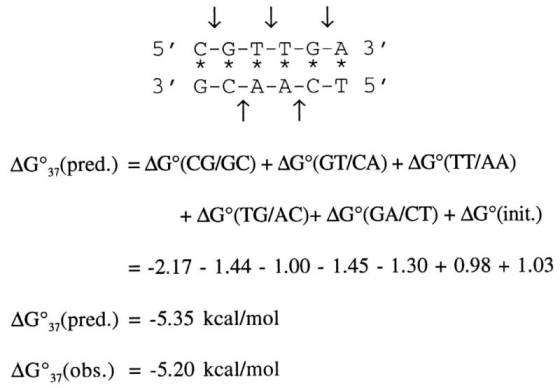
\includegraphics{NN}
\caption
{
C\'{a}lculo de estabilidad (energ\'{i}a libre de Gibbs, $\Delta G$) a temperatura fisiol\'{o}gica en base al modelo NN, 
incluyendo un t\'{e}rmino de iniciaci\'{o}n de d\'{u}plex, tomado de \citep{SantaLucia1998}.
Copyright (1998) National Academy of Sciences.
}
\label{fig:NN}
\end{center}
\end{figure}

Inspir\'{a}ndose en estructuras moleculares conocidas, 
este tipo de modelos se han empleado para describir la lectura indirecta del DNA, por su forma, 
por parte de nucleosomas \citep{Heijden2012} o factores de transcripci\'{o}n \citep{Gromiha2004,Espinosa2008}.

\begin{figure}
\begin{center} 
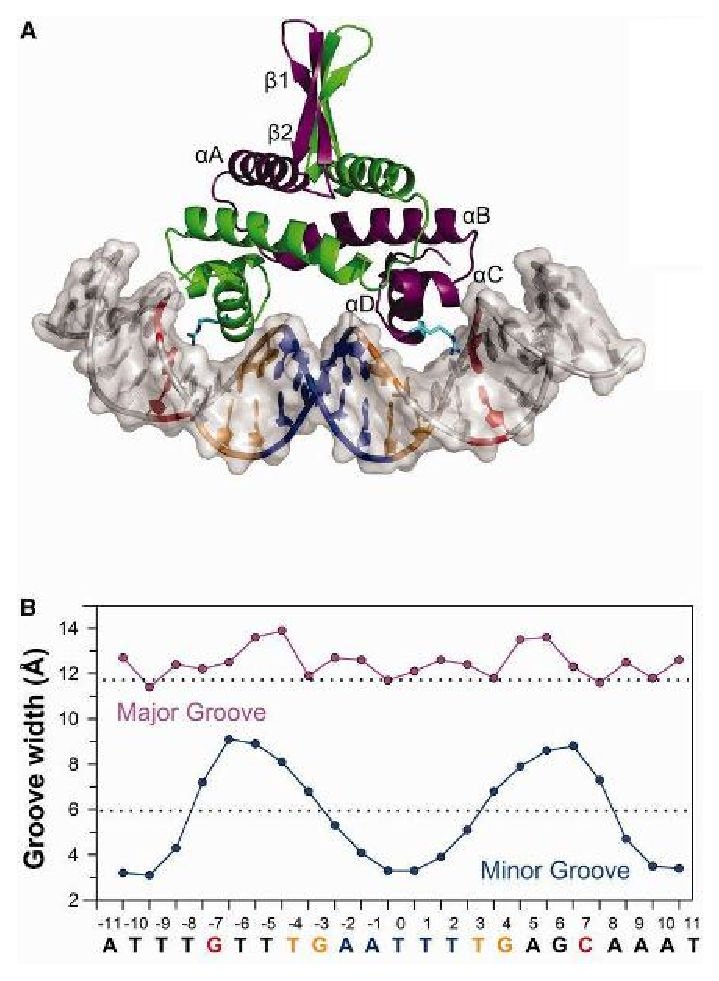
\includegraphics{MGW}
\caption
{
(A) Estructura de un homod\'{i}mero de Fis unido a un sitio de alta afinidad 
(PDB: \htmladdnormallink{3IV5}{http://www.rcsb.org/structure/3IV5}), 
insertando dos h\'{e}lices en dos surcos mayores consecutivos. 
(B) Ancho del surco mayor (magenta) y menor (MGW, azul) a lo largo de la secuencia de DNA medido entre los fosfatos m\'{a}s cercanos.
Las lineas punteadas representan los valores can\'{o}nicos para B-DNA. 
Figura adaptada de \citet{Hancock2013} y reproducida con permiso de los autores.
}
\label{fig:MGW}
\end{center}
\end{figure}

\begin{figure}
\begin{center} 
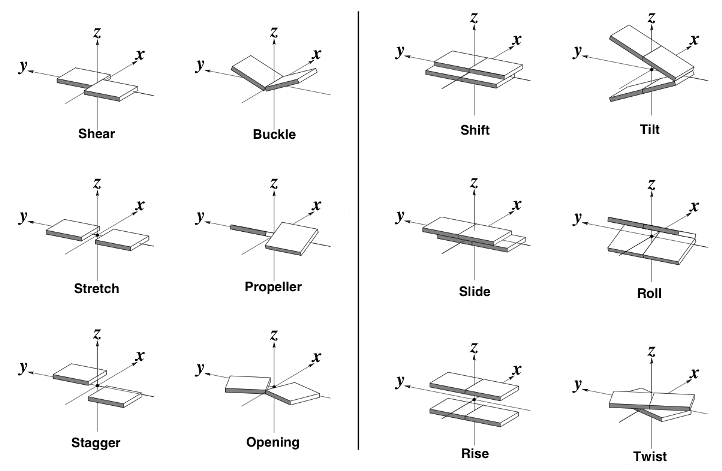
\includegraphics{BPgeom}
\caption
{
Propiedades de pares de bases (izquierda) y dinucle\'{o}tidos (derecha) que se pueden estimar a partir de la estructura. 
Figura tomada de \htmladdnormallink{x3dna.org}{http://x3dna.org/articles/seeing-is-understanding-as-well-as-believing}.
}
\label{fig:BPgeometry}
\end{center}
\end{figure}

%\begin{figure}
%\begin{center} 
%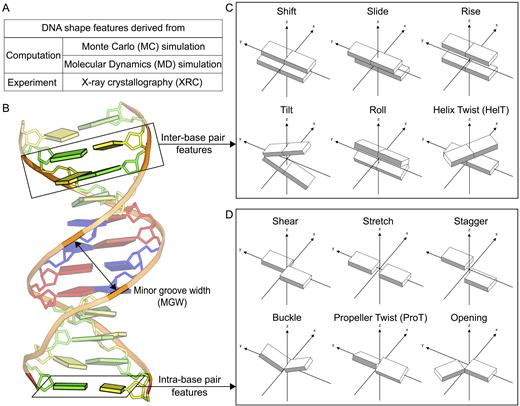
\includegraphics{DNAshape13}
%\caption{Propiedades de pares de bases y dinucle\'{o}tidos que se pueden estimar a partir de la estructura \citep{Li2017}.}
%\label{fig:DNAshape13}
%\end{center}
%\end{figure}



Otros modelos ampl\'{i}an el n\'{u}mero de vecinos considerados hasta llegar, por ejemplo, a pent\'{a}meros:

\begin{figure}
\begin{center} 
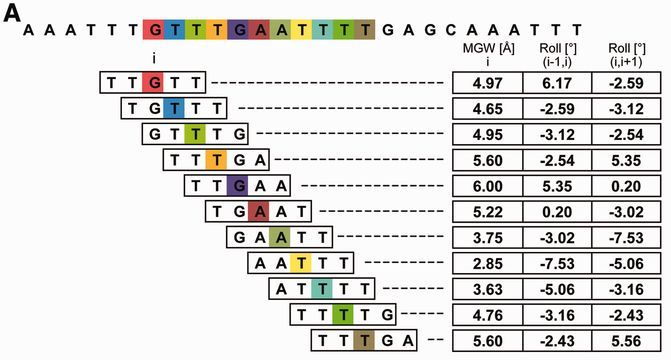
\includegraphics{DNApentamers}
\caption
{
Aproximaci\'{o}n de propiedades estructurales (MGW=minor groove width) de un d\'{u}plex de ADN por solapamiento de pent\'{a}meros, 
base del algoritmo \htmladdnormallink{DNAshape}{http://rohsdb.cmb.usc.edu}. 
Reproducido con permiso de \citet{Zhou2013}.
Este tipo de aproximaciones se est\'{a}n usando para enriquecer motivos de DNA reconocidos por factores de transcripci\'{o}n \citep{Yang2015}.
}
\label{fig:NN5}
\end{center}
\end{figure}

En esta secci\'{o}n aplicaremos el modelo NN a la predicci\'{o}n de promotores:

\begin{itemize}
\item \textbf{PROBLEMA:} disponemos de coordenadas gen\'{o}micas de una colecci\'{o}n de marcos de lectura 
(\htmladdnormallink{\italics{Open Reading Frames, ORFs}}{http://es.wikipedia.org/wiki/Marco_abierto_de_lectura}), 
pero desconocemos la posici\'{o}n de sus secuencias promotoras
\item \textbf{SOLUCI\'{O}N PROPUESTA:} buscar los promotores en la secuencia del DNA por su menor estabilidad termodin\'{a}mica
\end{itemize}

Este problema ha tenido mayor importancia en procariotas por la gran velocidad con que se han ido obteniendo sus secuencias gen\'{o}micas, 
y el algoritmo de \cite{Kanhere2005} es un ejemplo de como emplear una estrategia estructural para atacar este problema. 
El algoritmo consiste en estimar la estabilidad helicoidal del ADN cromos\'{o}mico, que se supone es menor en
las regiones promotoras, donde la maquinaria transcripcional se asienta para comenzar la s\'{i}ntesis de ARN. 
En concreto este m\'{e}todo estima la estabilidad de una (ventana de) secuencia de ADN a ambos lados de una coordenada y define como posibles
posiciones promotores aquellas donde la diferencia de estabilidad en torno a una coordenada es significativa. 

\begin{figure}
\begin{center} 
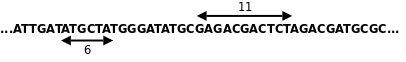
\includegraphics{window}
\caption
{
Ejemplos de ventanas de 6 y 11 nucle\'{o}tidos, que sirven para promediar propiedades a lo largo de la secuencia.
}
\label{fig:window}
\end{center}
\end{figure}

Este algoritmo incluye varios par\'{a}metros libres y en el art\'{i}culo original se muestra como entrenarlo para obtener valores adecuados para todos ellos.

\begin{figure}
\begin{center} 
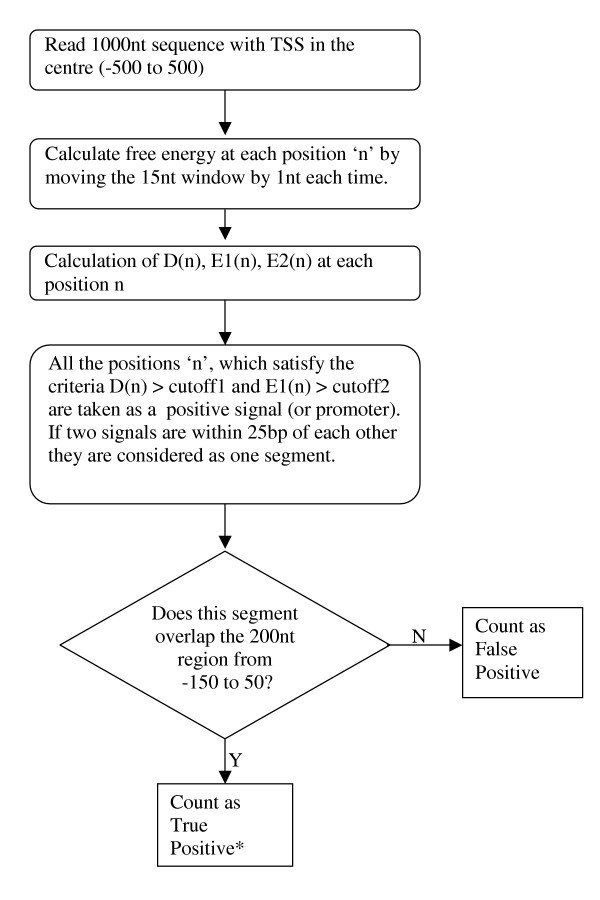
\includegraphics{flowKanhere}
\caption
{
Algoritmo de \cite{Kanhere2005}, que se basa en calcular la diferencia de $\Delta G$ entre dos ventanas en torno a una posici\'{o}n $n$.
Figura reproducida con permiso de los autores.
}
\label{fig:Kanhere}
\end{center}
\end{figure}

Se han propuesto otras aproximaciones estructurales, como la de \cite{Gogni2007}, %(\htmladdnormallink{PDF}{./papers/euk_promoter_prediction2007.pdf})
que identifica regiones promotoras en base a la capacidad de deformaci\'{o}n de los 
\htmladdnormallink{pares de bases}{http://nar.oxfordjournals.org/content/31/17/5108/F1.large.jpg},
estimada por medio de extensas simulaciones moleculares precalculadas. 
%Sin duda \'{e}sta es un \'{a}rea de investigaci\'{o}n en crecimiento y constantemente se siguen publicando 
%\htmladdnormallink{nuevos trabajos}{http://www.ncbi.nlm.nih.gov/pubmed?term=structural[All Fields] AND prediction[All Fields] AND promoters[All Fields]}. 

El repertorio de m\'{e}todos para predicci\'{o}n de promotores en base a inferencias estructurales es limitado, pero incluye al menos: 
\htmladdnormallink{proStar}{http://mmb.pcb.ub.es/proStar/}, \htmladdnormallink{ProSOM}{http://bioinformatics.psb.ugent.be/software/details/ProSOM}
%\htmladdnormallink{profisi}{http://mlg.ucd.ie/profisi} 
o el algoritmo de \citet{Song2012}. Otras opciones recientes se basan en combinar diferentes fuentes por medio de algoritmos de aprendizaje \citep{Eser2016}.

El ejercicio de esta secci\'{o}n consiste en completar el siguiente programa, usando los par\'{a}metros unificados de \cite{SantaLucia1998},
para calcular la diferencia de estabilidad $D(n)$ entre dos fragmentos de 50bp y 100bp $E1(n)$ y $E2(n)$ 
que flanquean una regi\'{o}n central (de 50bp) que podr\'{i}a albergar el promotor.
A su vez, estos framentos se calculan sobre valores de estabilidad calculados sobre ventanas de secuencia 
de longitud 15pb en el art\'{i}culo de \cite{Kanhere2005}:

\begin{equation}
E1(n) = \frac{\sum_{n}^{n+49}\Delta G}{50} 
\end{equation}

\begin{equation}
E2(n) = \frac{\sum_{n+99}^{n+199}\Delta G}{100} 
\end{equation}

\begin{equation}
D(n) = E1(n) - E2(n)
\end{equation}

Como conjunto de datos para la predicci\'{o}n de promotores usaremos las secuencias del fichero \htmladdnormallink{K12\_400\_50\_sites}{./files/K12_400_50_sites}, 
que contiene coordenadas de ORFs de \italics{Escherichia coli} con coordenadas -400,+50, con el 0 centrado cerca del cod\'{o}n de inicio.
Qu\'{e} observas al cambiar el tama\~no de la ventana?
\verbatiminput{code/prog1.1.pl}
\section{Dise\~no de primers para PCR} \label{dna2}

La reacci\'{o}n en cadena de la polimerasa 
(\htmladdnormallink{PCR}{http://es.wikipedia.org/wiki/Reacci\%C3\%B3n_en_cadena_de_la_polimerasa})
es una metodolog\'{i}a est\'{a}ndar en cualquier laboratorio de biolog\'{i}a molecular y consta fundamentalmente
de 3 fases que se repiten un n\'{u}mero de ciclos dentro de un tubo de ensayo que se encuentra en un ba\~{n}o:

\begin{figure}
\begin{center} 
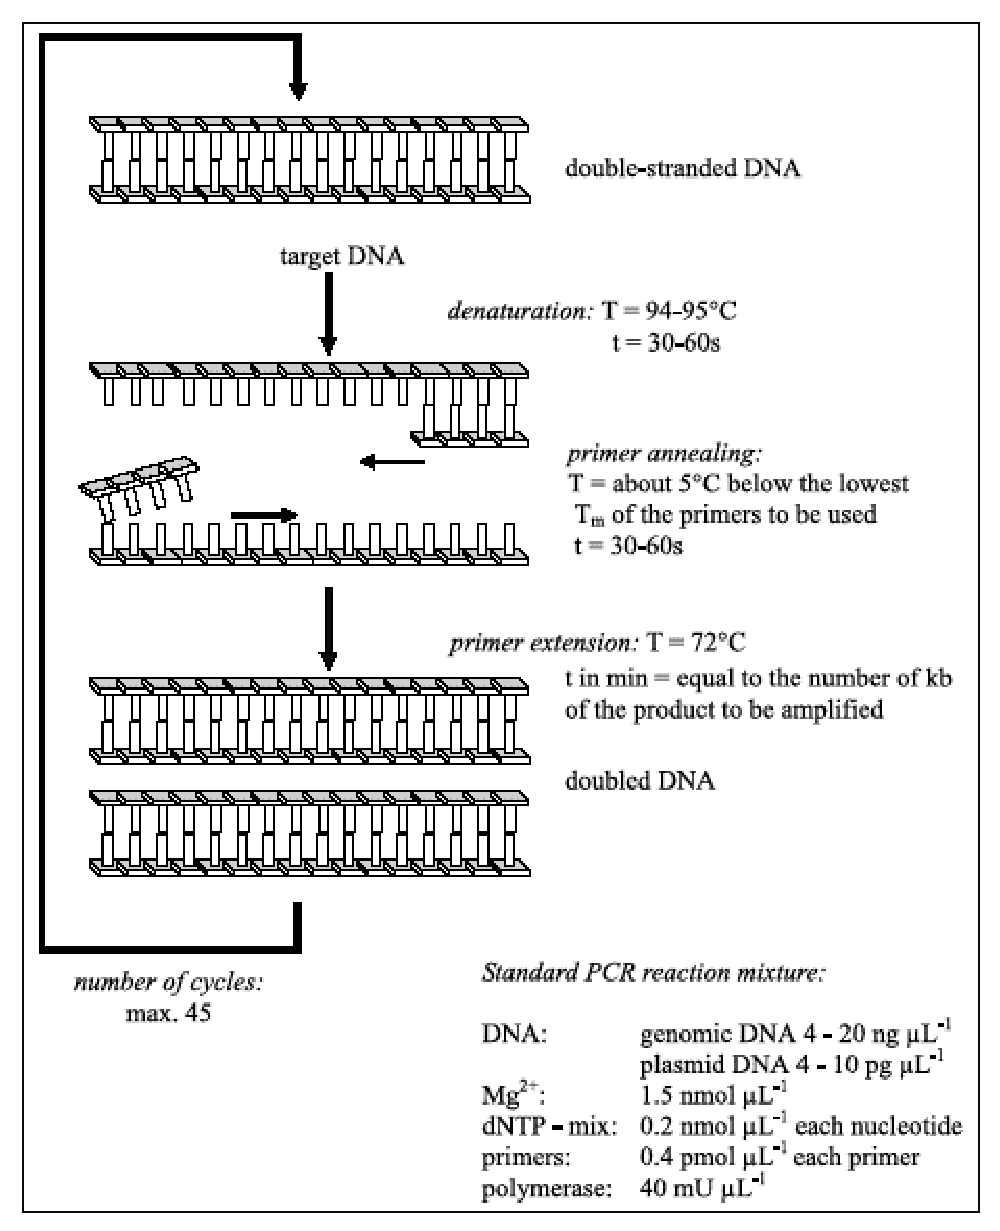
\includegraphics{PCR}
\caption
{
Diagrama de flujo de una reacci\'{o}n de PCR, 
que consiste en ciclos donde se repiten 3 fases: desnaturalizaci\'{o}n, apareamiento y elongaci\'{o}n.
En la primera el ADN se desnaturaliza separ\'{a}ndose las dos hebras.
En la segunda los cebadores o primers se hibridan con las hebras de ADN en posiciones donde las 
secuencias son complementarias y se forman puentes de H entre bases enfrentadas. 
Es una renaturalizaci\'{o}n parcial que se hace ajustando la temperatura a la secuencia de los cebadores. 
Finalmente, en la tercera etapa se ajusta la temperatura para favorecer la extensi\'{o}n de la nueva hebra
a partir de los cebadores por parte de la polimerasa. 
El tiempo de extensi\'{o}n es proporcional a la longitud del producto de PCR (o amplic\'{o}n) esperado
en funci\'{o}n de los cebadores dise\~{n}ados por el usuario y el genoma en cuesti\'{o}n.
Figura de \cite{Konietzny2003} reproducida con permiso de los autores.
}
\label{fig:PCR}
\end{center}
\end{figure}

Para cada aplicaci\'{o}n de la PCR es necesario ajustar las condiciones y el dise\~no de la reacci\'{o}n,
por ejemplo:
\begin{itemize} 
\item la duraci\'{o}n de las fases de apareamiento y elongaci\'{o}n
\item el tipo de cebadores o \italics{primers} empleados y sus temperaturas de fusi\'{o}n $T_{m}$ (ver secci\'{o}n \ref{desnat})
\item el tipo de polimerasa utilizada
\item las cantidad de los reactivos y de ADN molde
\item la longitud del amplic\'{o}n o producto de PCR obtenido
\end{itemize}

En esta secci\'{o}n veremos algunos de los algoritmos habituales para el dise\~no de cebadores, 
que deben cumplir al menos tres condiciones: 

%PCR Nearly Always Works and Design Is Not that Important
%Different Methods for Predicting Hybridization Tm Are Essentially Equivalent in Accuracy
%Designing Forward and Reverse Primers to Have Matching Tm\u2019s Is the Best Strategy to Optimize for PCR
%\u201cPrimer Dimer\u201d Artifacts Are Due to Dimerization of Primers
%A BLAST Search Is the Best Method for Determining the Specificity of a Primer
%At the End of PCR, Amplification Efficiency Is Not Exponential Because the Primers or NTPs Are Exhausted or the Polymerase Looses Activity
%Multiplex PCR Can Succeed by Optimization of Individual PCRs

%Aunque hay variaciones seg\'{u}n el uso, los primers se dise\~nan para cumplir con ciertas 
%\htmladdnormallink{condiciones}{http://www.bioquest.org/bioinformatics/module/cooper/Primer_Design/primer_design.htm}:
%; estas temperaturas suelen ser $T_{a} > 55$, lo 
%que se traduce en valores de GC cercanos al 50\% y longitudes entre 17 y 28 nucle\'{o}tidos

\begin{itemize} \label{reqprimers}
\item Una pareja de cebadores debe tener temperaturas de alineamiento muy cercanas para maximizar el rendimiento, 
lo cual suele traducirse en un contenido en GC similar, entre 50\% y 60\%. 
\item Los primers no deben favorecer horquillas (\italics{hairpins}) ni ser complementarios. 
El siguiente esquema muestra un cebador con una horquilla potencial a la izquierda y un par de cebadores que se aparean a la derecha:
\begin{verbatim}
          5'GGGAAA                    5' GGGAAAATTCCAGGATCTAT 3'
             |||| )                       ||||  ||||
 3' TATCTAGGACCTTA            3' TATCTAGGACCTTAAAAGGG 5'     
\end{verbatim}
\item Tras analizar una gran colecci\'{o}n de primers publicados en la literatura, parece que conviene evitar secuencias 
que terminen en GGG,GGT,ATT,CGA,TAA o TTA \citep{Onodera2007}.
\end{itemize}

Hay muchos programas que pueden ayudar en el dise\~no de primers en la web, como por ejemplo:
\begin{itemize}
\item \htmladdnormallink{primer3}{http://bioinfo.ut.ee/primer3/}
\item \htmladdnormallink{Vector NTI}{http://en.wikipedia.org/wiki/Vector_NTI}
\item \emph{in silico} PCR en \htmladdnormallink{procariotas}{http://insilico.ehu.es/PCR/} 
	y en \htmladdnormallink{animales}{http://genome.ucsc.edu/cgi-bin/hgPcr} 
\end{itemize}

o estos otros para dise\~nar primers degenerados, que permiten reconocer y por tanto amplificar varias secuencias similares
\begin{itemize}
%\item \htmladdnormallink{CODEHOP}{http://blocks.fhcrc.org/codehop.html} (sin mantenimiento)%https://icodehop.cphi.washington.edu/i-codehop-context/Welcome} 
\item \htmladdnormallink{amplicon}{http://amplicon.sourceforge.net/} 
\item \htmladdnormallink{primers4clades}{http://maya.ccg.unam.mx/primers4clades/} (espec\'{i}fico para aplicaciones filogen\'{e}ticas, utiliza CODEHOP)
\end{itemize}

Sin embargo, m\'{a}s all\'{a} del software elegido, es importante saber c\'{o}mo se calculan ciertas propiedades moleculares de los primers,
para poder analizar con criterio los resultados obtenidos. 

Por ejemplo, nos puede interesar calcular la $T_{m}$, 
que es la temperatura a la que la mitad de los primers se han hibridado con el ADN molde, 
o la cantidad de ADN bicatenario a cualquier temperatura, por ejemplo a la temperatura de apareamiento, 
la m\'{a}s cr\'{i}tica, que a menudo se aproxima como $T_{m} - 5$.

Una aproximaci\'{o}n burda es llamada regla de Wallace, que se basa solamente en la secuencia,
donde GC y AT son el n\'{u}mero de nucle\'{o}tidos G/C y A/T en la secuencia del cebador, respectivamente \citep{Santalucia2007}:
\begin{equation}
T_{m} \sim 4GC + 2AT
\end{equation}

Otra alternativa m\'{a}s precisa es la siguiente ecuaci\'{o}n, 
que relaciona exactamente la temperatura con la proporci\'{o}n de ADN bicatenario,
donde $[A]$ es la concentraci\'{o}n de hebras en exceso (los primers), $[B]$ el ADN molde que queremos amplificar,
$\Delta H$ el cambio de entalp\'{i}a, $\Delta S$ el cambio de entrop\'{i}a y $R$ la 
\htmladdnormallink{constante de Boltzmann}{http://en.wikipedia.org/wiki/Boltzmann_constant} (R=1.987 cal/mol K):
\begin{equation}
T_{m} = \frac{1000 \Delta H}{\Delta S + Rln([A]-\frac{[B]}{2})} - 273.15
\end{equation}

%\begin{figure}
%\begin{center} 
%
\includegraphics{TvsC}
%\caption{Curva te\'{o}rica que muestra la dependencia entre temperatura y [ADN hibridado], tomada de \citep{Santalucia2007}.}
%\label{fig:TvsC}
%\end{center}
%\end{figure}

En la pr\'{a}ctica combinamos esta ecuaci\'{o}n con el modelo \italics{Nearest Neighbor} (NN, secci\'{o}n \ref{dna1}), 
usando valores experimentales de entalp\'{i}a y entrop\'{i}a obtenidos para dinucle\'{o}tidos.

Con el objetivo de probar estas recetas el siguiente ejercicio incluye:
\begin{itemize}
\item usar cualquier software que conozcas (o de los citados arriba) para dise\~nar varios primers
\item con ayuda del siguiente c\'{o}digo Python evaluar parejas de primers teniendo en cuenta su $T_{m}$ 
de fusi\'{o}n y su potencial de formaci\'{o}n de horquillas
\item compara las $T_{m}$ obtenidas con las que resultan de aplicar la regla de Wallace
\item prueba a modificar el c\'{o}digo para calcular temperaturas de alineamiento donde la proporci\'{o}n
de primer hibridado sea por ejemplo del 95\%
\verbatiminput{code/prog1.2.py}
\end{itemize}
